\documentclass{article}
\usepackage{graphicx}
\usepackage[margin=1.5cm]{geometry}
\usepackage{amsmath}

\begin{document}

\title{Tuesday Reading Assessment: Unit 5, Forces}
\author{Prof. Jordan C. Hanson}

\maketitle

\section{Memory Bank}

\begin{itemize}
\item Force of drag, in air or other gas: $F_D = \frac{1}{2}C \rho A v^2$.
\item In the above formula, $C$ is an empirical constant, $\rho$ is the density of the air or gas, $A$ is the area of the object, and $v$ is the object's velocity.
\end{itemize}
\begin{figure}[ht]
\centering
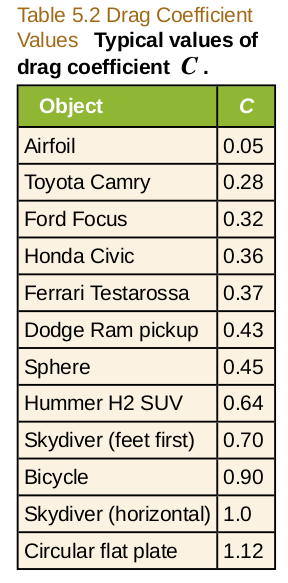
\includegraphics[width=0.2\textwidth]{drag.png}
\caption{\label{fig:drag} A table of drag coefficients, C.}
\end{figure}
\section{Chapter 5 - Drag}
\begin{enumerate}
\item Suppose a Toyota Camry and a Honda Civic are street racing.  Each has been modified to be capable of speeds of 50 m/s ($\approx 180$ km/h).  (a) Assuming each model has the same cross-sectional area, $A$, which model experiences a higher drag force? (b) Given that $\rho = 1.2$ kg/m$^3$, $A = 4.0$ m$^2$, and $v=40$ m/s, what is the drag force on each? \\ \vspace{2cm}
\item If the driver of the Honda Civic decreases the speed by a factor of 2 (down to $20$ m/s), what is the new drag force?
\end{enumerate}

\end{document}
